\chapter{Especificación de Requisitos Funcionales y No Funcionales}

\section{Requisitos funcionales}
Los requisitos funcionales de una herramienta o aplicación, describen cualquier comportamiento o funcionalidad concreta de la misma, bajo ciertas circunstancias. De una manera genérica, los requisitos funcionales deben incluir las acciones que realizan las pantallas específicas de la interfaz o describir cada uno de los flujos de datos y computo de cada una de las capas de la herramienta.

En este apartado, se van a dividir los requisitos funcionales en distintos grupos según la capa del software.

\subsection{Requisitos funcionales de cómputo (Nivel inferior)}
Lo primero de todo es comprobar que funcionalidad se realiza en el nivel más inferior del sistema. Esto permitirá tener una idea global de lo que hace el sistema. 
\begin{itemize}
	\item Cuando se ejecuta uno de los paquetes que contienen el código fuente para realizar los cálculos de cada uno de los gráficos, o el paquete para obtener un resumen sobre un fichero, lo primero que hace Spark es buscar dicho archivo, en la ruta especificada, dentro del HDFS.
	\item Los archivos que contiene los datos deben ser tipo CSV.
	\item La conexión Spark-Hadoop se realiza mediante una librería específica para realizar estas acciones, dentro de Spark.
	\item Una vez recuperado el archivo, el siguiente paso es transformarlo en un Dataframe, la estructura con la que trabaja Spark para tratar los datos.
	\item Antes de continuar con los cálculos, se crean las estructuras que almacenarán los datos resultados en formato JSON, dependiendo del paquete que se esté ejecutando.
	\item A continuación, se aplica el esquema de agrupación y la técnica de reducción de datos elegida para cada uno de los gráficos.
	\item En el caso de la librería encargada de extraer los datos resumen o ‘summary’, se encarga de obtener datos propios del archivo como el número de columnas, el número de filas, el peso del archivo o los nombres de todas las columnas.
	\item Una vez obtenidos los resultados, estos se almacenan en las estructuras indicadas anteriormente. 
	\item Después, se realiza la comunicación entre Spark y MongoDB para guardar estos resultados dentro de una base de datos y colección indicados en los parámetros.
\end{itemize}

\subsection{Requisitos funcionales de comunicación (Nivel intermedio)}
\begin{itemize}
	\item El sistema se encargará de crear el servidor virtual donde se gestionarán todas las peticiones por parte de la interfaz web.
	\item Todas las peticiones que recibe se gestionan de manera asíncrona, lo que permite realizar múltiples acciones a la vez.
	\item Los parámetros de conexión con Hadoop, Spark y MongoDB están configurados en este nivel y, por el momento, solo son accesibles a través de código.
	\item Cuando el sistema solicite obtener el contenido de un path especifico dentro del HDFS de Hadoop, NodeJS enviará una solicitud a la API RESTful de Hadoop, donde se obtiene como resultado un listado, en formato JSON, de todos los documentos y directorios que existen dentro del indicado, con información importante de cada uno.
	\item Esta información devuelta será mostrada en los campos indicados para ello en la interfaz web.
	\item Cuando se solicite un nuevo gráfico en la interfaz web, se recogerá como una petición asíncrona de tipo 'get'.
	\item Justo después, se creará un identificador para cada una de las solicitudes de gráficos, compuesta por la ruta del archivo, el peso del mismo, el gráfico seleccionado y los parámetros.
	\item Cada una de las variables que componen el identificador, se encripta utilizando MD5. 
	\item Se debe crear un documento de tipo JSON, que se almacenará en una colección dentro de la base de datos de MongoDB, el cual servirá para mantener información, como la hora de inicio y fin de la ejecución o el gráfico indicado, sobre los documentos solicitados y los resultados de los gráficos y de los datos proporcionados por ‘summay’. 
	\item Este identificador también se envía como parámetro al nivel inferior, para que pueda ser identificado el resultado de la agrupación devuelto por Spark.
	\item Según indique el usuario en la interfaz, este mismo resultado puede ser representado de manera gráfica o directamente visualizar los datos en formato JSON. 
	\item Si el usuario solicita un gráfico que ya ha sido generado anteriormente, el sistema no volverá a realizar el cálculo sobre el fichero indicado, sino que buscará primero con el identificador si ya está cargado en la base de datos de MongoDB el resultado, o si otro usuario lo ha solicitado pero todavía no está completado. En cuyo caso, deberá esperar hasta que esté disponible para recoger el resultado y pintar el gráfico.
\end{itemize}

\subsection{Requisitos funcionales de la interfaz gráfica (Nivel superior)}
Como se puede apreciar en la figura \ref{fig:interfazinicial}, la interfaz del usuario final es bastante sencilla y simple de usar. Toda la funcionalidad gráfica se muestra en una sola pantalla, para simplificar la búsqueda de los elementos.
\begin{figure}
	\centering
	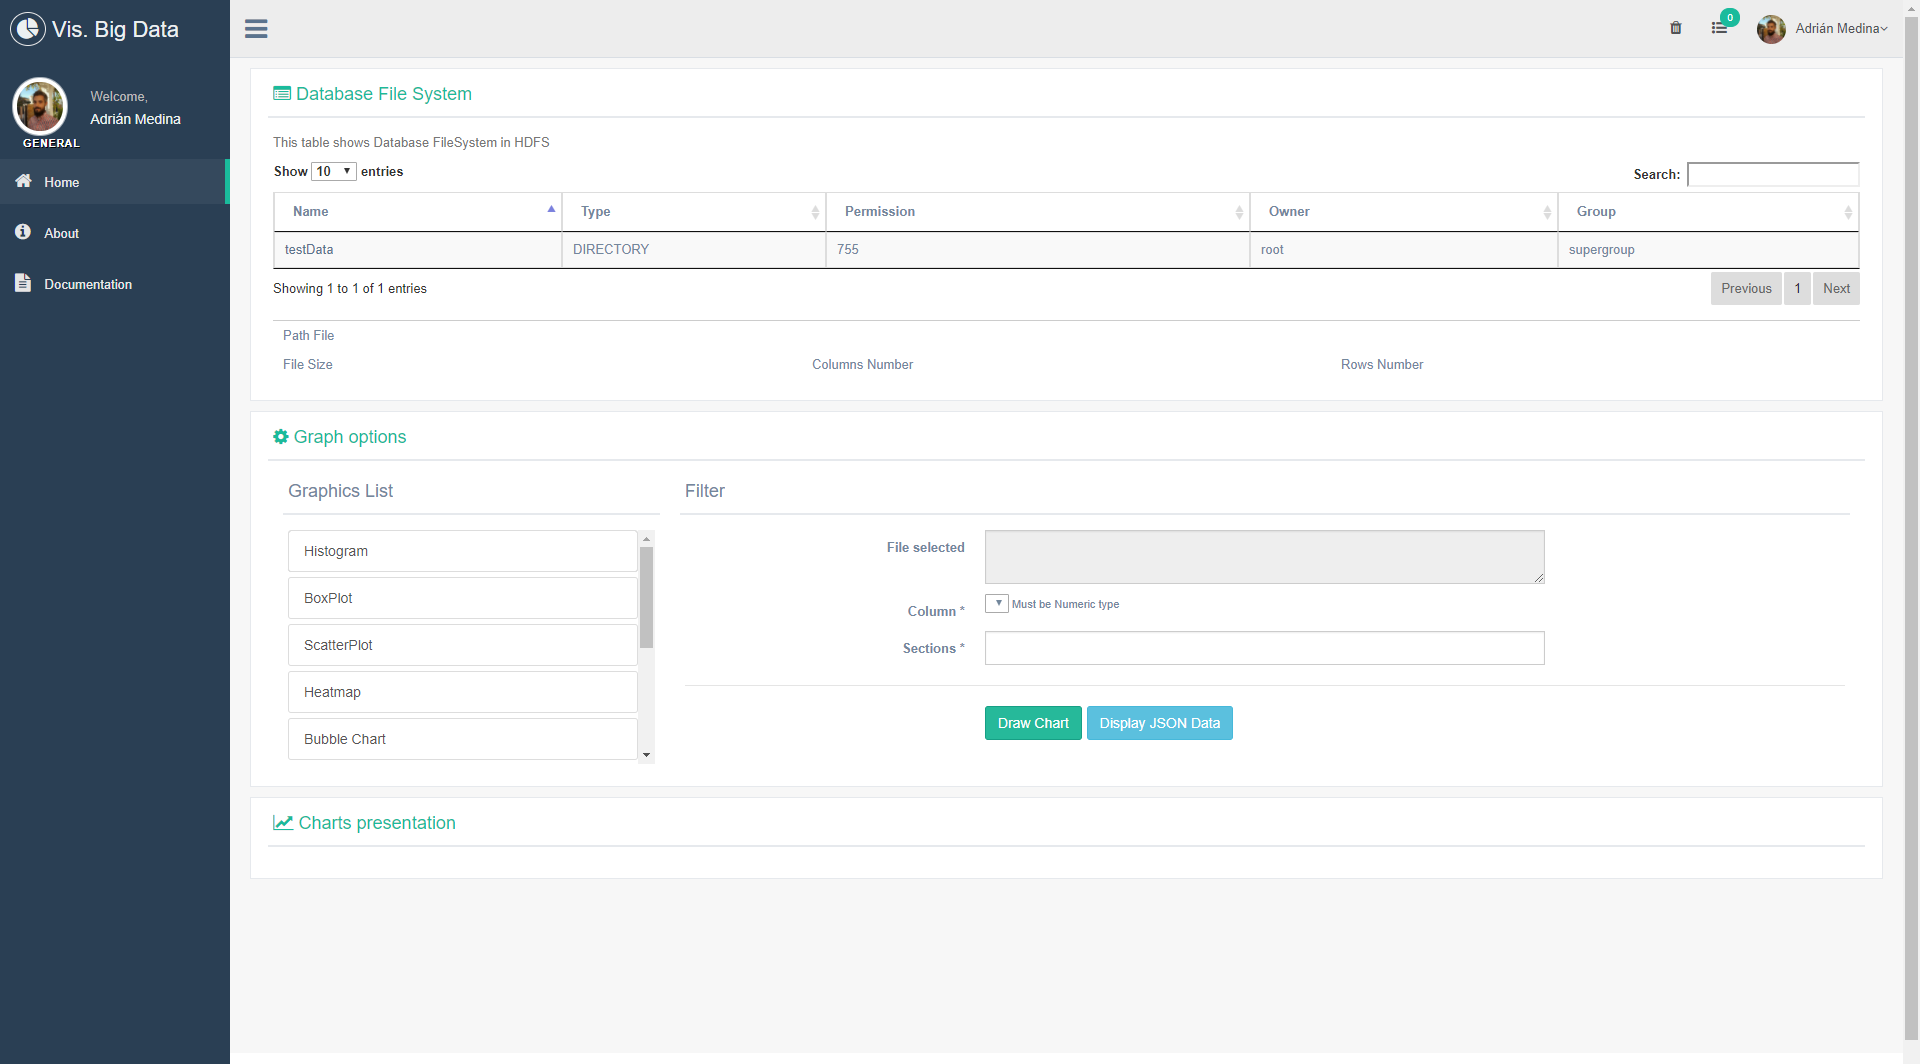
\includegraphics[width=1\linewidth]{imagenes/interfaz_inicial}
	\caption{Vista inicial de la interfaz web de la API}
	\label{fig:interfazinicial}
\end{figure}
\begin{figure}
	\centering
	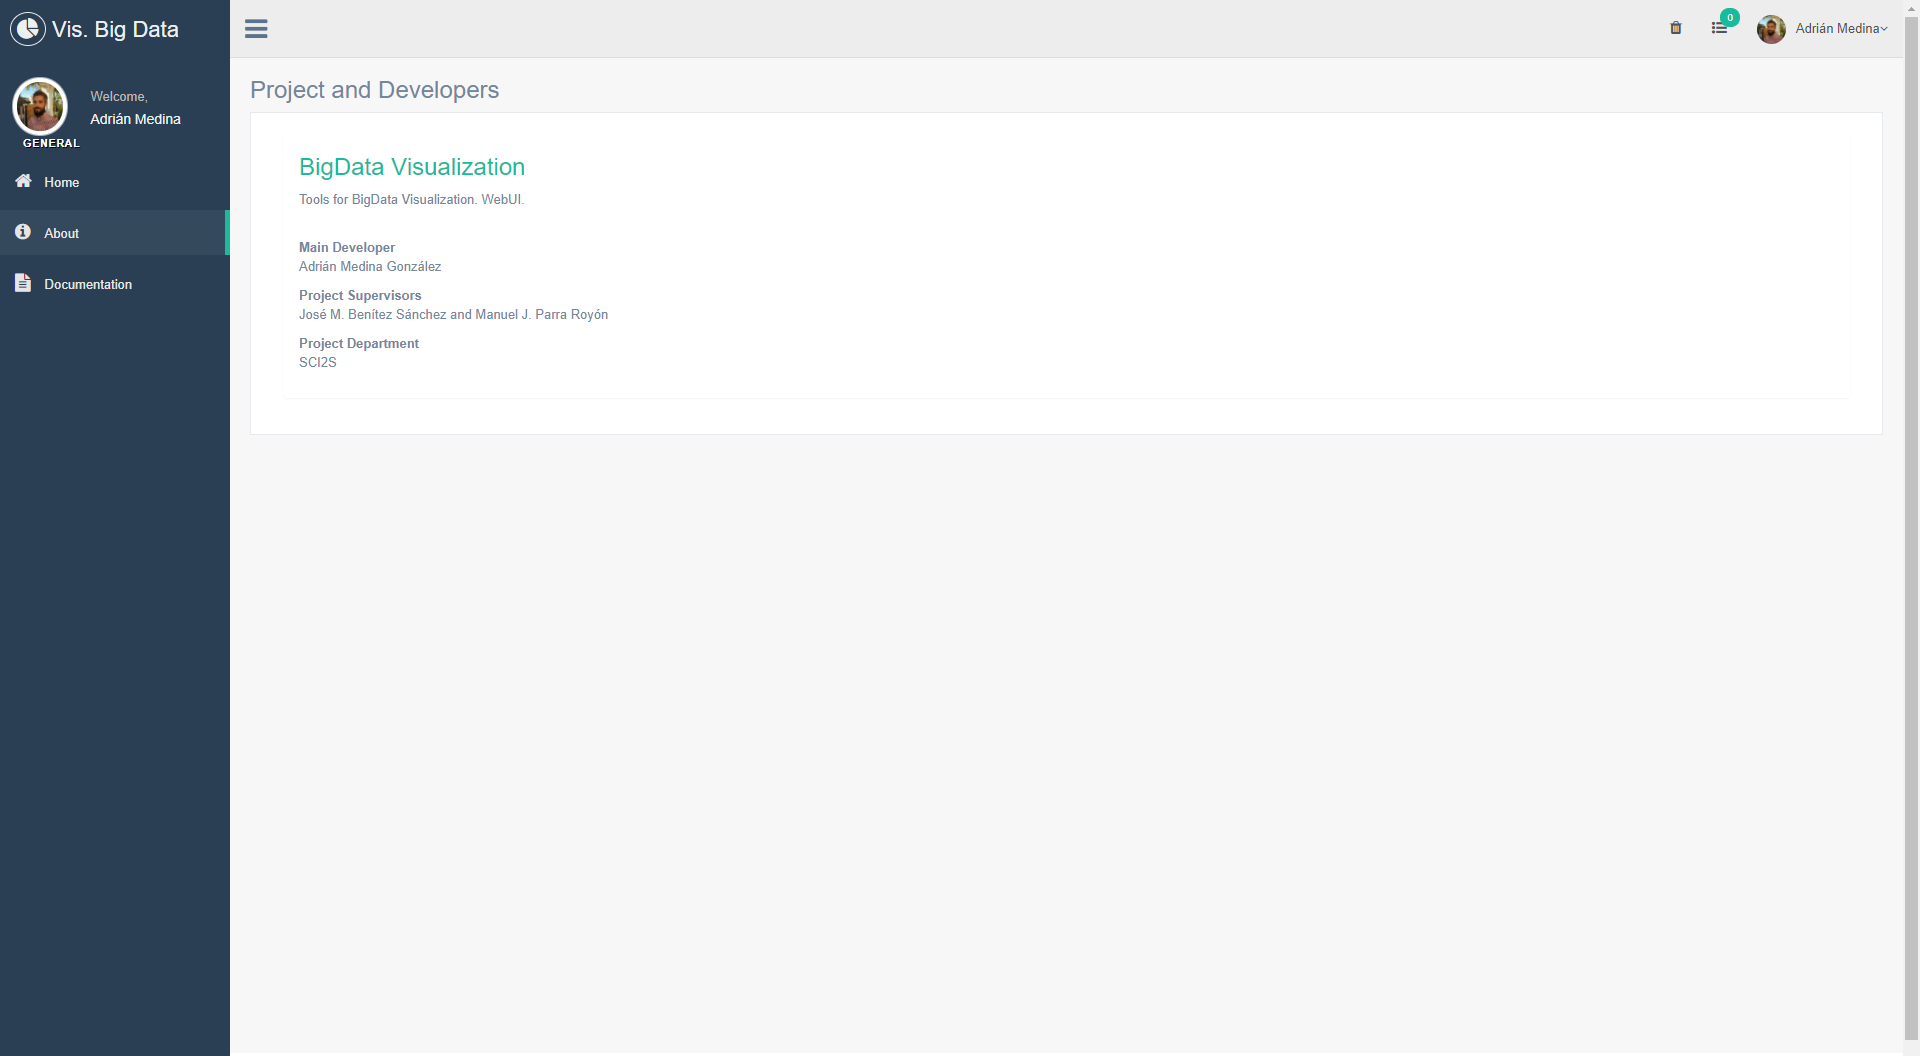
\includegraphics[width=1\linewidth]{imagenes/boton_about}
	\caption{Información sobre el proyecto}
	\label{fig:botonabout}
\end{figure}
\begin{figure}
	\centering
	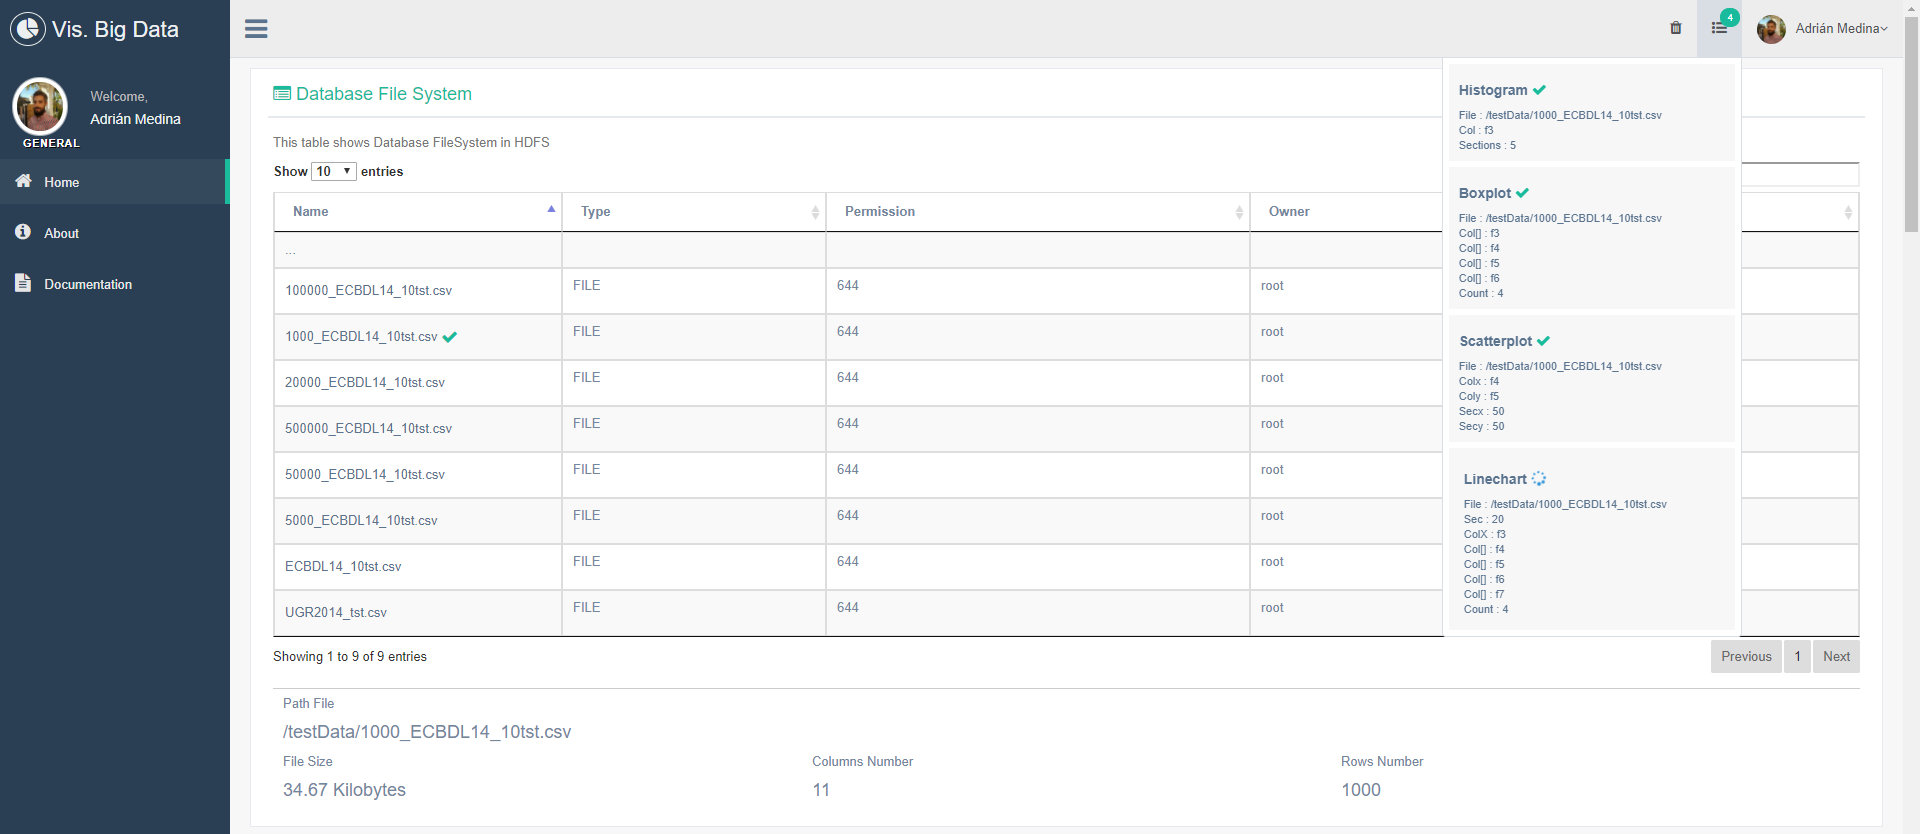
\includegraphics[width=1\linewidth]{imagenes/lista_ultimos_graficos}
	\caption{Listado de los últimos gráficos generados}
	\label{fig:listaultimosgraficos}
\end{figure}

\begin{itemize}
	\item Al cargar la interfaz, el sistema cargará automáticamente el contenido del directorio raíz del HDFS, en la sección indicada para ello.
	\item En esta tabla se muestra información de los archivos y directorios de la ruta actual, como el nombre, si es un directorio o un archivo, los permisos que tiene dentro del HDFS, el usuario propietario y el grupo al que pertenece.
	\item Cada uno de los botones de la cabecera de la tabla permite ordenar el contenido de manera ascendente o descendente.
	\item Hay un menú desplegable donde se puede indicar el número de documentos que se desean visualizar en la tabla.
	\item Si hubiera más elementos de los indicados, el gestor de páginas de la tabla permite navegar entre las distintas listas de registros.
	\item En el campo ‘Search’, se puede buscar un registro concreto haciendo coincidir parte de la cadena que se escriba en el campo con algún contenido de los registros, de cualquier columna, ya sea el nombre, propietario o grupo, por ejemplo. Solo buscará los ficheros o directorios que se encuentren en el directorio actual que se está mostrando.
	\item Si el registro es un directorio, al hacer click en él, el sistema se encargará de obtener el contenido del mismo y actualizar la tabla con los nuevos registros.
	\item Por el contrario, si se trata de un fichero de tipo CSV, mandará a NodeJS la petición de obtener el resultado de ejecutar ‘summary’.
	\item Si se trata de un fichero de otro tipo o el fichero seleccionado se encuentra vacío, el sistema mostrará un mensaje de error indicando que es un fichero invalido.
	\item El resultado de ‘summary’ se mostrará en los campos habilitados para ello (justo debajo de la tabla donde se muestran los registros del HDFS).
	\item En el panel ‘Graph options’, el sistema muestra una lista de todos los gráficos disponibles en la herramienta. 
	\item Al seleccionar uno, el sistema habilitará un formulario para rellenar con los parámetros que necesita ese gráfico para calcular el resultado del nivel inferior.
	\item El sistema rellenará automáticamente los campos de ‘File selected’ y los campos de las columnas y ejes, con los datos obtenidos al seleccionar un fichero en la tabla del HDFS.
	\item Una vez relleno el formulario, al pinchar en el botón ‘Draw Chart’, se le comunicará a NodeJS la petición con los parámetros indicados, y devolverá el gráfico resultado en el panel ‘Charts presentation’. 
	\item Si por el contrario seleccionamos el botón ‘Display JSON Data’, en vez de dibujar el gráfico, mostrará los datos en formato JSON.
	\item En este último panel, se pueden acumular tantos gráficos como se ejecuten, con la posibilidad de comparar varios a la vez, teniendo la posibilidad de cerrar alguno haciendo click en el símbolo ‘X’ de la esquina superior derecha.
	\item En la parte superior de la pantalla, el sistema almacena una lista tanto con los últimos gráficos que se han generado como los que se están ejecutando actualmente, como se puede apreciar en la figura \ref{fig:listaultimosgraficos}. De esta manera, si se selecciona uno que ya esté finalizado, el sistema ejecutará de nuevo el gráfico con los mismos parámetros sin la necesidad de volver a introducirlos a mano.
	\item El botón justo a la izquierda, con el icono del cubo, ejecuta la función de limpiado de la lista, si después de ejecutar muchos gráficos, el usuario necesita tenerla vacía.
	\item También arriba a la derecha se encuentra información sobre el usuario y algunas de las acciones que se podrán hacer, cuando se implemente en un futuro la gestión de usuarios.
	\item En el menú lateral izquierdo, el botón ‘Home’ y el título del proyecto justo encima, ejecuta la pantalla principal con el contenido descrito anteriormente.
	\item El botón ‘About’, muestra información acerca del proyecto, como una breve descripción de la funcionalidad de la API, su desarrollador principal o supervisores del proyecto, tal y como se muestra en la figura \ref{fig:botonabout}.
	\item El botón 'Documentation' abre una nueva ventana con la API RESTful que proporciona Swagger, donde se puede obtener información acerca de todas las funcionalidades del sistema, como se puede apreciar en la figura \ref{fig:swaggerfunciones}.
	\item Si se selecciona una de las funciones, se puede ejecutar para obtener el resultado en formato JSON, indicándole los parámetros necesarios, tal y como se puede ver en un ejemplo sobre la función encargada del histograma en la figura \ref{fig:swaggerhistograma}.
	\item Al hacer click en cualquiera de los botones del menú lateral izquierdo, el sistema hace una recarga de la página para mostrar su contenido.
\end{itemize}

\begin{figure}
	\centering
	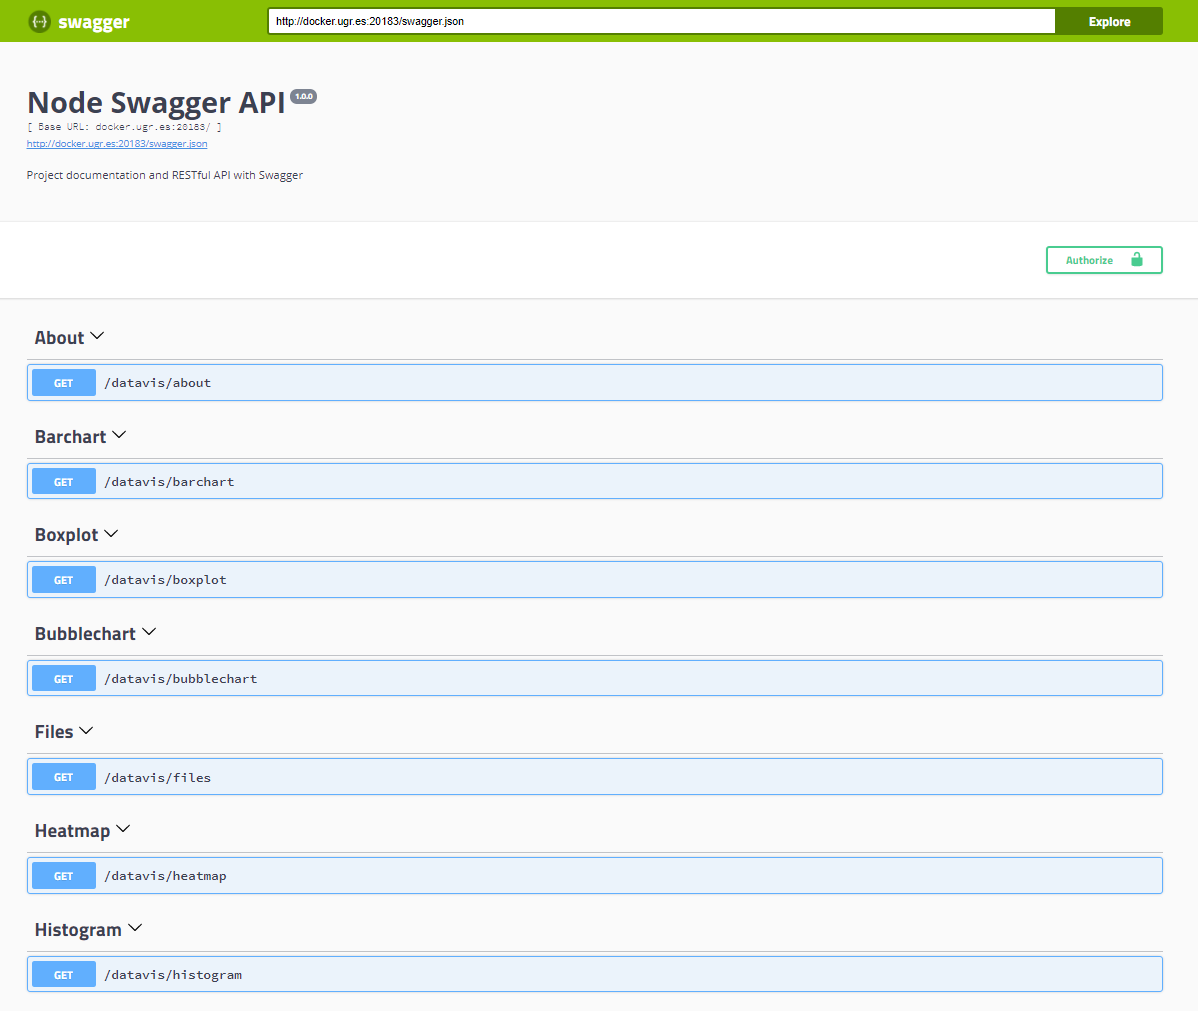
\includegraphics[width=1\linewidth]{imagenes/swagger_funciones}
	\caption{Funciones a través de Swagger}
	\label{fig:swaggerfunciones}
\end{figure}
\begin{figure}
	\centering
	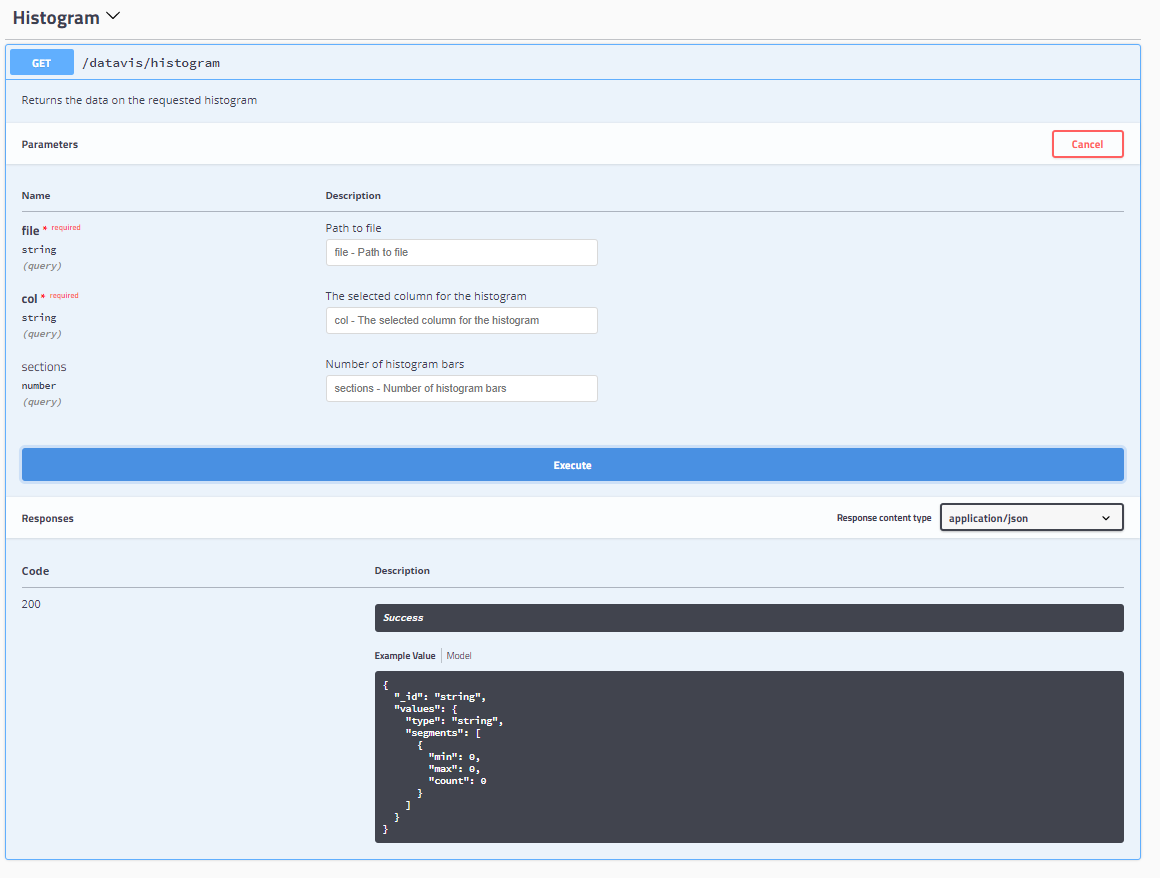
\includegraphics[width=1\linewidth]{imagenes/swagger_histograma}
	\caption{Función histograma en Swagger}
	\label{fig:swaggerhistograma}
\end{figure}

\section{Requisitos no funcionales}
Los requisitos no funcionales representan características de funcionamiento y algunas restricciones del sistema que se está implementando. Estos requisitos no se refieren al comportamiento específico de las funciones del sistema, sino características del propio sistema como la concurrencia, la escalabilidad o eficiencia. De esta forma, podemos agruparlos según las características.

\subsection{Eficiencia}
\begin{itemize}
	\item El sistema debe ejecutar las peticiones de manera asíncrona, por lo que permite usar la herramienta en varios dispositivos, obteniendo cada uno sus propios resultados.
	\item Por la misma razón, el sistema debe ser capaz de operar con muchos usuarios al mismo tiempo de manera fluida.
	\item Si el cálculo de un gráfico concreto, sobre el mismo fichero y con los mismos parámetros ya ha sido ejecutado anteriormente, entonces no volverá a realizar la misma operación, agilizando así la fluidez con la que se obtienen los resultados en la API.
	\item El sistema debe cargar de manera veloz los directorios del HDFS de Hadoop, para no aumentar los tiempos de espera de la API.
	\item Todos los cambios que se realicen sobre los ficheros en el HDFS, deben estar listos al instante para poder generar los gráficos con los nuevos datos.
	\item El sistema debe ser capaz de recibir y ejecutar varias peticiones a la vez sin problemas.
	\item Spark y Scala deben aprovechar al máximo los recursos del ordenador o cluster disponibles al permitir dividir y ejecutar los procesos en paralelo.
\end{itemize}

\subsection{Escalabilidad}
\begin{itemize}
	\item Al estar montado el sistema sobre herramientas fácilmente escalables como Hadoop o Spark, debe permitir instalarlo y ejecutarlo sobre cualquier ordenador o cluster, tanto en el aumento de nodos como en su decremento.
	\item Por el mismo motivo anterior, al cambiar de componentes hardware debe seguir funcionando perfectamente, siempre que cumpla los requisitos mínimos del sistema.
\end{itemize}

\subsection{Seguridad de los datos}
\begin{itemize}
	\item El sistema tiene copias de seguridad gracias a la estructura de almacenamiento de datos de Hadoop gracias a HDFS.
	\item Los datos resultados permanecen en MongoDB con su correspondiente documento con información acerca del estado de los mismos.
\end{itemize}

\subsection{Accesibilidad}
\begin{itemize}
	\item El sistema tiene compatibilidad con cualquier navegador web actualizado en sus últimas versiones.
	\item También la interfaz está diseñada para adaptarse a los tamaños de los dispositivos móviles o tablets, actualizados recientemente.
\end{itemize}

\subsection{Requisitos hardware}
\begin{itemize}
	\item Es necesario tener instaladas y configuradas las herramientas Hadoop, Spark, MongoDB y NodeJS
	\item El sistema debe poder lanzar el HDFS de Hadoop en el sistema, que requiere como mínimo 8 GB de RAM.
	\item Como mínimo, el sistema ocupa cerca de los 4GB de disco.
	\item En el caso de Spark y MongoDB, los requisitos hardware son los configurados para estas herramientas, ya que se puede ejecutar desde un ordenador hasta un cluster. 
\end{itemize}

\subsection{Versiones}
\begin{itemize}
	\item El sistema debe tener instalado una versión de Java JDK igual o superior a 1.7.0
	\item La versión de Scala debe ser 2.11
	\item Para Hadoop, tener instalado como mínimo la versión 2.6
	\item Se ha configurado Spark para utilizar una versión igual o superior a 2.0
	\item Debe instalarse y configurarse igual o superior de MongoDB a la 3.2
	\item Para NodeJS, la versión debe ser 6.9 o superior
	\item También es necesario tener otras aplicaciones secundarias como Sbt, Swagger y Forever para el correcto funcionamiento de la aplicación.
\end{itemize}


